\documentclass[twoside]{book}

% Packages required by doxygen
\usepackage{fixltx2e}
\usepackage{calc}
\usepackage{doxygen}
\usepackage[export]{adjustbox} % also loads graphicx
\usepackage{graphicx}
\usepackage[utf8]{inputenc}
\usepackage{makeidx}
\usepackage{multicol}
\usepackage{multirow}
\PassOptionsToPackage{warn}{textcomp}
\usepackage{textcomp}
\usepackage[nointegrals]{wasysym}
\usepackage[table]{xcolor}

% NLS support packages
\usepackage[italian]{babel}

% Font selection
\usepackage[T1]{fontenc}
\usepackage[scaled=.90]{helvet}
\usepackage{courier}
\usepackage{amssymb}
\usepackage{sectsty}
\renewcommand{\familydefault}{\sfdefault}
\allsectionsfont{%
  \fontseries{bc}\selectfont%
  \color{darkgray}%
}
\renewcommand{\DoxyLabelFont}{%
  \fontseries{bc}\selectfont%
  \color{darkgray}%
}
\newcommand{\+}{\discretionary{\mbox{\scriptsize$\hookleftarrow$}}{}{}}

% Page & text layout
\usepackage{geometry}
\geometry{%
  a4paper,%
  top=2.5cm,%
  bottom=2.5cm,%
  left=2.5cm,%
  right=2.5cm%
}
\tolerance=750
\hfuzz=15pt
\hbadness=750
\setlength{\emergencystretch}{15pt}
\setlength{\parindent}{0cm}
\setlength{\parskip}{3ex plus 2ex minus 2ex}
\makeatletter
\renewcommand{\paragraph}{%
  \@startsection{paragraph}{4}{0ex}{-1.0ex}{1.0ex}{%
    \normalfont\normalsize\bfseries\SS@parafont%
  }%
}
\renewcommand{\subparagraph}{%
  \@startsection{subparagraph}{5}{0ex}{-1.0ex}{1.0ex}{%
    \normalfont\normalsize\bfseries\SS@subparafont%
  }%
}
\makeatother

% Headers & footers
\usepackage{fancyhdr}
\pagestyle{fancyplain}
\fancyhead[LE]{\fancyplain{}{\bfseries\thepage}}
\fancyhead[CE]{\fancyplain{}{}}
\fancyhead[RE]{\fancyplain{}{\bfseries\leftmark}}
\fancyhead[LO]{\fancyplain{}{\bfseries\rightmark}}
\fancyhead[CO]{\fancyplain{}{}}
\fancyhead[RO]{\fancyplain{}{\bfseries\thepage}}
\fancyfoot[LE]{\fancyplain{}{}}
\fancyfoot[CE]{\fancyplain{}{}}
\fancyfoot[RE]{\fancyplain{}{\bfseries\scriptsize Generato da Doxygen }}
\fancyfoot[LO]{\fancyplain{}{\bfseries\scriptsize Generato da Doxygen }}
\fancyfoot[CO]{\fancyplain{}{}}
\fancyfoot[RO]{\fancyplain{}{}}
\renewcommand{\footrulewidth}{0.4pt}
\renewcommand{\chaptermark}[1]{%
  \markboth{#1}{}%
}
\renewcommand{\sectionmark}[1]{%
  \markright{\thesection\ #1}%
}

% Indices & bibliography
\usepackage{natbib}
\usepackage[titles]{tocloft}
\setcounter{tocdepth}{3}
\setcounter{secnumdepth}{5}
\makeindex

% Hyperlinks (required, but should be loaded last)
\usepackage{ifpdf}
\ifpdf
  \usepackage[pdftex,pagebackref=true]{hyperref}
\else
  \usepackage[ps2pdf,pagebackref=true]{hyperref}
\fi
\hypersetup{%
  colorlinks=true,%
  linkcolor=blue,%
  citecolor=blue,%
  unicode%
}

% Custom commands
\newcommand{\clearemptydoublepage}{%
  \newpage{\pagestyle{empty}\cleardoublepage}%
}

\usepackage{caption}
\captionsetup{labelsep=space,justification=centering,font={bf},singlelinecheck=off,skip=4pt,position=top}

%===== C O N T E N T S =====

\begin{document}

% Titlepage & ToC
\hypersetup{pageanchor=false,
             bookmarksnumbered=true,
             pdfencoding=unicode
            }
\pagenumbering{roman}
\begin{titlepage}
\vspace*{7cm}
\begin{center}%
{\Large S\+OL -\/ S\+P\+A\+R\+SE \\[1ex]\large 1 }\\
\vspace*{1cm}
{\large Generato da Doxygen 1.8.11}\\
\end{center}
\end{titlepage}
\clearemptydoublepage
\tableofcontents
\clearemptydoublepage
\pagenumbering{arabic}
\hypersetup{pageanchor=true}

%--- Begin generated contents ---
\chapter{Indice dei tipi composti}
\section{Elenco dei tipi composti}
Queste sono le classi, le struct, le union e le interfacce con una loro breve descrizione\+:\begin{DoxyCompactList}
\item\contentsline{section}{\hyperlink{structelem}{elem} }{\pageref{structelem}}{}
\item\contentsline{section}{\hyperlink{structsmatrix__t}{smatrix\+\_\+t} }{\pageref{structsmatrix__t}}{}
\end{DoxyCompactList}

\chapter{Indice dei file}
\section{Elenco dei file}
Questo è un elenco dei file documentati con una loro breve descrizione\+:\begin{DoxyCompactList}
\item\contentsline{section}{\hyperlink{client_8c}{client.\+c} \\*Semplice client di test }{\pageref{client_8c}}{}
\item\contentsline{section}{{\bfseries connections.\+h} }{\pageref{connections_8h}}{}
\item\contentsline{section}{\hyperlink{icl__hash_8c}{icl\+\_\+hash.\+c} }{\pageref{icl__hash_8c}}{}
\item\contentsline{section}{\hyperlink{icl__hash_8h}{icl\+\_\+hash.\+h} }{\pageref{icl__hash_8h}}{}
\item\contentsline{section}{\hyperlink{membox_8c}{membox.\+c} \\*File principale del server membox }{\pageref{membox_8c}}{}
\item\contentsline{section}{\hyperlink{message_8h}{message.\+h} \\*Contiene il formato del messaggio }{\pageref{message_8h}}{}
\item\contentsline{section}{\hyperlink{ops_8h}{ops.\+h} \\*Contiene i codici delle operazioni di richiesta e risposta }{\pageref{ops_8h}}{}
\item\contentsline{section}{{\bfseries stats.\+h} }{\pageref{stats_8h}}{}
\end{DoxyCompactList}

\chapter{Documentazione delle classi}
\hypertarget{structelem}{}\section{Riferimenti per la struct elem}
\label{structelem}\index{elem@{elem}}


{\ttfamily \#include $<$sparse.\+h$>$}



Diagramma di collaborazione per elem\+:\nopagebreak
\begin{figure}[H]
\begin{center}
\leavevmode
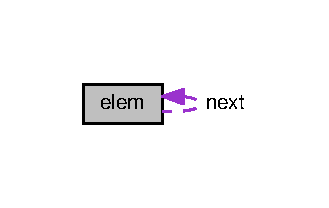
\includegraphics[width=158pt]{structelem__coll__graph}
\end{center}
\end{figure}
\subsection*{Attributi pubblici}
\begin{DoxyCompactItemize}
\item 
unsigned \hyperlink{structelem_aca409f3a7c1c9621b262a230c78ef37b}{col}
\item 
double \hyperlink{structelem_a52a0b099052bdf7611aa32acdb3f5449}{val}
\item 
struct \hyperlink{structelem}{elem} $\ast$ \hyperlink{structelem_ab9cf5c2e1c9a0ec2938275b90d39d5ca}{next}
\end{DoxyCompactItemize}


\subsection{Descrizione dettagliata}
Le matrici sparse di valori double sono rappresentate da un array di liste ciascuna delle quali rappresenta una riga. In ogni lista sono contenuti solo gli elementi non uguali a zero con il numero di colonna corrispondente.

Ad esempio la matrice

3.\+1 0 0 0 0 0 0 0 0 7.\+2 0 9.\+0

è rappresentata come

0 $\vert$ ------$>$(\mbox{[}0,3.\+1\mbox{]} , N\+U\+LL) 1 $\vert$ N\+U\+LL 2 $\vert$ ------$>$(\mbox{[}1,7.\+2\mbox{]} , --)--$>$( \mbox{[}3,9.\+0\mbox{]} ,N\+U\+LL)elemento della matrice sparsa 

\subsection{Documentazione dei membri dato}
\index{elem@{elem}!col@{col}}
\index{col@{col}!elem@{elem}}
\subsubsection[{\texorpdfstring{col}{col}}]{\setlength{\rightskip}{0pt plus 5cm}unsigned elem\+::col}\hypertarget{structelem_aca409f3a7c1c9621b262a230c78ef37b}{}\label{structelem_aca409f3a7c1c9621b262a230c78ef37b}
indice di colonna \index{elem@{elem}!next@{next}}
\index{next@{next}!elem@{elem}}
\subsubsection[{\texorpdfstring{next}{next}}]{\setlength{\rightskip}{0pt plus 5cm}struct {\bf elem}$\ast$ elem\+::next}\hypertarget{structelem_ab9cf5c2e1c9a0ec2938275b90d39d5ca}{}\label{structelem_ab9cf5c2e1c9a0ec2938275b90d39d5ca}
puntatore al prossimo elemento nella riga \index{elem@{elem}!val@{val}}
\index{val@{val}!elem@{elem}}
\subsubsection[{\texorpdfstring{val}{val}}]{\setlength{\rightskip}{0pt plus 5cm}double elem\+::val}\hypertarget{structelem_a52a0b099052bdf7611aa32acdb3f5449}{}\label{structelem_a52a0b099052bdf7611aa32acdb3f5449}
valore dell\textquotesingle{}elemento 

La documentazione per questa struct è stata generata a partire dal seguente file\+:\begin{DoxyCompactItemize}
\item 
\hyperlink{sparse_8h}{sparse.\+h}\end{DoxyCompactItemize}

\hypertarget{structsmatrix__t}{}\section{Riferimenti per la struct smatrix\+\_\+t}
\label{structsmatrix__t}\index{smatrix\+\_\+t@{smatrix\+\_\+t}}


{\ttfamily \#include $<$sparse.\+h$>$}



Diagramma di collaborazione per smatrix\+\_\+t\+:\nopagebreak
\begin{figure}[H]
\begin{center}
\leavevmode
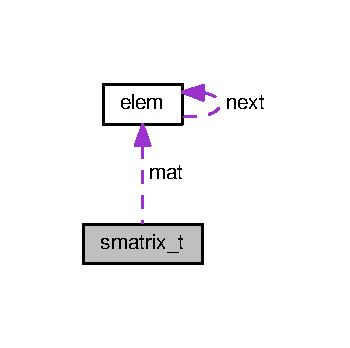
\includegraphics[width=168pt]{structsmatrix__t__coll__graph}
\end{center}
\end{figure}
\subsection*{Attributi pubblici}
\begin{DoxyCompactItemize}
\item 
\hyperlink{sparse_8h_a14aec81bdea9c2d34b666b7157117387}{elem\+\_\+t} $\ast$$\ast$ \hyperlink{structsmatrix__t_aa60ccb45be474ec81f6daab4fcdab2c4}{mat}
\item 
int \hyperlink{structsmatrix__t_ae0b8f31ddab7ed23ca14a46758291f37}{nrow}
\item 
int \hyperlink{structsmatrix__t_a7a7218430298fc18a42dfa43ecc41635}{ncol}
\end{DoxyCompactItemize}


\subsection{Descrizione dettagliata}
rappresentazione della matrice sparsa 

\subsection{Documentazione dei membri dato}
\index{smatrix\+\_\+t@{smatrix\+\_\+t}!mat@{mat}}
\index{mat@{mat}!smatrix\+\_\+t@{smatrix\+\_\+t}}
\subsubsection[{\texorpdfstring{mat}{mat}}]{\setlength{\rightskip}{0pt plus 5cm}{\bf elem\+\_\+t}$\ast$$\ast$ smatrix\+\_\+t\+::mat}\hypertarget{structsmatrix__t_aa60ccb45be474ec81f6daab4fcdab2c4}{}\label{structsmatrix__t_aa60ccb45be474ec81f6daab4fcdab2c4}
puntatore all\textquotesingle{}array delle righe \index{smatrix\+\_\+t@{smatrix\+\_\+t}!ncol@{ncol}}
\index{ncol@{ncol}!smatrix\+\_\+t@{smatrix\+\_\+t}}
\subsubsection[{\texorpdfstring{ncol}{ncol}}]{\setlength{\rightskip}{0pt plus 5cm}int smatrix\+\_\+t\+::ncol}\hypertarget{structsmatrix__t_a7a7218430298fc18a42dfa43ecc41635}{}\label{structsmatrix__t_a7a7218430298fc18a42dfa43ecc41635}
numero di colonne \index{smatrix\+\_\+t@{smatrix\+\_\+t}!nrow@{nrow}}
\index{nrow@{nrow}!smatrix\+\_\+t@{smatrix\+\_\+t}}
\subsubsection[{\texorpdfstring{nrow}{nrow}}]{\setlength{\rightskip}{0pt plus 5cm}int smatrix\+\_\+t\+::nrow}\hypertarget{structsmatrix__t_ae0b8f31ddab7ed23ca14a46758291f37}{}\label{structsmatrix__t_ae0b8f31ddab7ed23ca14a46758291f37}
numero di righe 

La documentazione per questa struct è stata generata a partire dal seguente file\+:\begin{DoxyCompactItemize}
\item 
\hyperlink{sparse_8h}{sparse.\+h}\end{DoxyCompactItemize}

\chapter{Documentazione dei file}
\hypertarget{sparse_8c}{}\section{Riferimenti per il file sparse.\+c}
\label{sparse_8c}\index{sparse.\+c@{sparse.\+c}}


prototipi implementati  


{\ttfamily \#include \char`\"{}sparse.\+h\char`\"{}}\\*
{\ttfamily \#include $<$errno.\+h$>$}\\*
{\ttfamily \#include $<$stdlib.\+h$>$}\\*
{\ttfamily \#include $<$string.\+h$>$}\\*
Grafo delle dipendenze di inclusione per sparse.\+c\+:\nopagebreak
\begin{figure}[H]
\begin{center}
\leavevmode
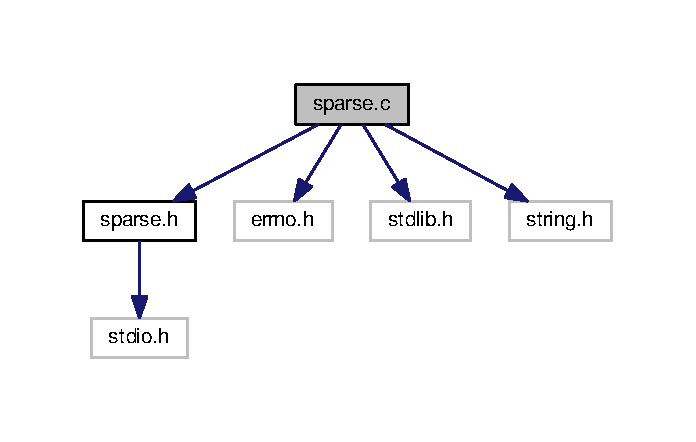
\includegraphics[width=334pt]{sparse_8c__incl}
\end{center}
\end{figure}
\subsection*{Funzioni}
\begin{DoxyCompactItemize}
\item 
\hyperlink{structsmatrix__t}{smatrix\+\_\+t} $\ast$ \hyperlink{sparse_8c_a13f7785dace4a2981b9b6f810ca34115}{new\+\_\+smat} (unsigned n, unsigned m)
\item 
\hyperlink{sparse_8h_a4ed992ceefff896353c1727143529d16}{bool\+\_\+t} \hyperlink{sparse_8c_a4232552afd0fdc736d90fded1f272759}{is\+\_\+equal\+\_\+smat} (\hyperlink{structsmatrix__t}{smatrix\+\_\+t} $\ast$a, \hyperlink{structsmatrix__t}{smatrix\+\_\+t} $\ast$b)
\item 
int \hyperlink{sparse_8c_a098b33ab9b543c109d655b9afc081bb7}{put\+\_\+elem\+\_\+row} (\hyperlink{sparse_8h_a14aec81bdea9c2d34b666b7157117387}{elem\+\_\+t} $\ast$$\ast$r, int j, double d)
\item 
int \hyperlink{sparse_8c_a19ab77e854480bb2c9e5032bc3f0ab9f}{put\+\_\+elem} (\hyperlink{structsmatrix__t}{smatrix\+\_\+t} $\ast$m, unsigned i, unsigned j, double d)
\item 
int \hyperlink{sparse_8c_a23f27b0ac759a8c6cf94ca624a7367d3}{get\+\_\+elem\+\_\+row} (\hyperlink{sparse_8h_a14aec81bdea9c2d34b666b7157117387}{elem\+\_\+t} $\ast$r, int j, double $\ast$pd)
\item 
int \hyperlink{sparse_8c_a03efbfc08da3aa936597103784ddbe45}{get\+\_\+elem} (\hyperlink{structsmatrix__t}{smatrix\+\_\+t} $\ast$m, unsigned i, unsigned j, double $\ast$pd)
\item 
void \hyperlink{sparse_8c_a58e3ead06f0ecc684dfc90538947343a}{free\+\_\+row} (\hyperlink{sparse_8h_a14aec81bdea9c2d34b666b7157117387}{elem\+\_\+t} $\ast$$\ast$pr)
\item 
void \hyperlink{sparse_8c_ad3596ce2e271a24fada5c85f3b8ce0af}{free\+\_\+smat} (\hyperlink{structsmatrix__t}{smatrix\+\_\+t} $\ast$$\ast$pm)
\item 
\hyperlink{structsmatrix__t}{smatrix\+\_\+t} $\ast$ \hyperlink{sparse_8c_afa8c4ca1cb9e4e55f40dd35faa1d9f85}{sum\+\_\+smat} (\hyperlink{structsmatrix__t}{smatrix\+\_\+t} $\ast$a, \hyperlink{structsmatrix__t}{smatrix\+\_\+t} $\ast$b)
\item 
\hyperlink{structsmatrix__t}{smatrix\+\_\+t} $\ast$ \hyperlink{sparse_8c_a633a6b934732ad44f5cf73e9c55c54e9}{prod\+\_\+smat} (\hyperlink{structsmatrix__t}{smatrix\+\_\+t} $\ast$a, \hyperlink{structsmatrix__t}{smatrix\+\_\+t} $\ast$b)
\item 
\hyperlink{structsmatrix__t}{smatrix\+\_\+t} $\ast$ \hyperlink{sparse_8c_a7b9192596db334fe30a652e05ab45987}{transp\+\_\+smat} (\hyperlink{structsmatrix__t}{smatrix\+\_\+t} $\ast$a)
\item 
\hyperlink{structsmatrix__t}{smatrix\+\_\+t} $\ast$ \hyperlink{sparse_8c_ac5049cd89f46bff8cd028382edf931e6}{load\+\_\+smat} (F\+I\+LE $\ast$fd)
\item 
int \hyperlink{sparse_8c_a9ee2597119d106f30a1ba43ba3d6c642}{save\+\_\+smat} (F\+I\+LE $\ast$fd, \hyperlink{structsmatrix__t}{smatrix\+\_\+t} $\ast$mat)
\item 
\hyperlink{structsmatrix__t}{smatrix\+\_\+t} $\ast$ \hyperlink{sparse_8c_a1bb39d59a532967d5f507a19700aafb1}{loadbin\+\_\+smat} (F\+I\+LE $\ast$fd)
\item 
int \hyperlink{sparse_8c_a8529b8bb59f8d259731ef88e5deb6d57}{savebin\+\_\+smat} (F\+I\+LE $\ast$fd, \hyperlink{structsmatrix__t}{smatrix\+\_\+t} $\ast$mat)
\end{DoxyCompactItemize}


\subsection{Descrizione dettagliata}
prototipi implementati 

\begin{DoxyAuthor}{Autore}
Francesco Lorito 464604 
\end{DoxyAuthor}


\subsection{Documentazione delle funzioni}
\index{sparse.\+c@{sparse.\+c}!free\+\_\+row@{free\+\_\+row}}
\index{free\+\_\+row@{free\+\_\+row}!sparse.\+c@{sparse.\+c}}
\subsubsection[{\texorpdfstring{free\+\_\+row(elem\+\_\+t $\ast$$\ast$pr)}{free_row(elem_t **pr)}}]{\setlength{\rightskip}{0pt plus 5cm}void free\+\_\+row (
\begin{DoxyParamCaption}
\item[{{\bf elem\+\_\+t} $\ast$$\ast$}]{pr}
\end{DoxyParamCaption}
)}\hypertarget{sparse_8c_a58e3ead06f0ecc684dfc90538947343a}{}\label{sparse_8c_a58e3ead06f0ecc684dfc90538947343a}
dealloca tutta la riga di una matrice


\begin{DoxyParams}{Parametri}
{\em pr} & puntatore al putatore della riga da deallocare ($\ast$pr viene messo a N\+U\+LL dalla funzione) \\
\hline
\end{DoxyParams}
\index{sparse.\+c@{sparse.\+c}!free\+\_\+smat@{free\+\_\+smat}}
\index{free\+\_\+smat@{free\+\_\+smat}!sparse.\+c@{sparse.\+c}}
\subsubsection[{\texorpdfstring{free\+\_\+smat(smatrix\+\_\+t $\ast$$\ast$pm)}{free_smat(smatrix_t **pm)}}]{\setlength{\rightskip}{0pt plus 5cm}void free\+\_\+smat (
\begin{DoxyParamCaption}
\item[{{\bf smatrix\+\_\+t} $\ast$$\ast$}]{pm}
\end{DoxyParamCaption}
)}\hypertarget{sparse_8c_ad3596ce2e271a24fada5c85f3b8ce0af}{}\label{sparse_8c_ad3596ce2e271a24fada5c85f3b8ce0af}
dealloca tutta la matrice


\begin{DoxyParams}{Parametri}
{\em pm} & puntatore al putatore della matrice da deallocare ($\ast$pm viene messo a N\+U\+LL dalla funzione) \\
\hline
\end{DoxyParams}
\index{sparse.\+c@{sparse.\+c}!get\+\_\+elem@{get\+\_\+elem}}
\index{get\+\_\+elem@{get\+\_\+elem}!sparse.\+c@{sparse.\+c}}
\subsubsection[{\texorpdfstring{get\+\_\+elem(smatrix\+\_\+t $\ast$m, unsigned i, unsigned j, double $\ast$pd)}{get_elem(smatrix_t *m, unsigned i, unsigned j, double *pd)}}]{\setlength{\rightskip}{0pt plus 5cm}int get\+\_\+elem (
\begin{DoxyParamCaption}
\item[{{\bf smatrix\+\_\+t} $\ast$}]{m, }
\item[{unsigned}]{i, }
\item[{unsigned}]{j, }
\item[{double $\ast$}]{pd}
\end{DoxyParamCaption}
)}\hypertarget{sparse_8c_a03efbfc08da3aa936597103784ddbe45}{}\label{sparse_8c_a03efbfc08da3aa936597103784ddbe45}
legge il valore nell\textquotesingle{}elemento i,j


\begin{DoxyParams}{Parametri}
{\em m} & puntatore alla matrice \\
\hline
{\em (i,j)} & posizione dell\textquotesingle{}elemento \\
\hline
{\em pd} & puntatore della variabile in cui scrivere il valore dell\textquotesingle{}elemento\\
\hline
\end{DoxyParams}

\begin{DoxyRetVals}{Valori di ritorno}
{\em -\/1} & se si e\textquotesingle{} verificato un errore \\
\hline
{\em 0} & altrimenti \\
\hline
\end{DoxyRetVals}
\index{sparse.\+c@{sparse.\+c}!get\+\_\+elem\+\_\+row@{get\+\_\+elem\+\_\+row}}
\index{get\+\_\+elem\+\_\+row@{get\+\_\+elem\+\_\+row}!sparse.\+c@{sparse.\+c}}
\subsubsection[{\texorpdfstring{get\+\_\+elem\+\_\+row(elem\+\_\+t $\ast$r, int j, double $\ast$pd)}{get_elem_row(elem_t *r, int j, double *pd)}}]{\setlength{\rightskip}{0pt plus 5cm}int get\+\_\+elem\+\_\+row (
\begin{DoxyParamCaption}
\item[{{\bf elem\+\_\+t} $\ast$}]{r, }
\item[{int}]{j, }
\item[{double $\ast$}]{pd}
\end{DoxyParamCaption}
)}\hypertarget{sparse_8c_a23f27b0ac759a8c6cf94ca624a7367d3}{}\label{sparse_8c_a23f27b0ac759a8c6cf94ca624a7367d3}
legge il valore dell\textquotesingle{}elemento nella colonna j


\begin{DoxyParams}{Parametri}
{\em r} & puntatore alla riga da leggere \\
\hline
{\em j} & colonna dell\textquotesingle{}elemento \\
\hline
{\em pd} & puntatore della variabile in cui scrivere il valore dell\textquotesingle{}elemento\\
\hline
\end{DoxyParams}

\begin{DoxyRetVals}{Valori di ritorno}
{\em -\/1} & se si e\textquotesingle{} verificato un errore \\
\hline
{\em 0} & altrimenti \\
\hline
\end{DoxyRetVals}
\index{sparse.\+c@{sparse.\+c}!is\+\_\+equal\+\_\+smat@{is\+\_\+equal\+\_\+smat}}
\index{is\+\_\+equal\+\_\+smat@{is\+\_\+equal\+\_\+smat}!sparse.\+c@{sparse.\+c}}
\subsubsection[{\texorpdfstring{is\+\_\+equal\+\_\+smat(smatrix\+\_\+t $\ast$a, smatrix\+\_\+t $\ast$b)}{is_equal_smat(smatrix_t *a, smatrix_t *b)}}]{\setlength{\rightskip}{0pt plus 5cm}{\bf bool\+\_\+t} is\+\_\+equal\+\_\+smat (
\begin{DoxyParamCaption}
\item[{{\bf smatrix\+\_\+t} $\ast$}]{a, }
\item[{{\bf smatrix\+\_\+t} $\ast$}]{b}
\end{DoxyParamCaption}
)}\hypertarget{sparse_8c_a4232552afd0fdc736d90fded1f272759}{}\label{sparse_8c_a4232552afd0fdc736d90fded1f272759}
Controlla se due matrici sono uguali, elemento per elemento


\begin{DoxyParams}{Parametri}
{\em a} & puntatore alla prima matrice da confrontare \\
\hline
{\em b} & puntatore alla seconda matrice da confrontare\\
\hline
\end{DoxyParams}

\begin{DoxyRetVals}{Valori di ritorno}
{\em T\+R\+UE} & se sono uguali \\
\hline
{\em F\+A\+L\+SE} & altrimenti \\
\hline
\end{DoxyRetVals}
\index{sparse.\+c@{sparse.\+c}!load\+\_\+smat@{load\+\_\+smat}}
\index{load\+\_\+smat@{load\+\_\+smat}!sparse.\+c@{sparse.\+c}}
\subsubsection[{\texorpdfstring{load\+\_\+smat(\+F\+I\+L\+E $\ast$fd)}{load_smat(FILE *fd)}}]{\setlength{\rightskip}{0pt plus 5cm}{\bf smatrix\+\_\+t}$\ast$ load\+\_\+smat (
\begin{DoxyParamCaption}
\item[{F\+I\+LE $\ast$}]{fd}
\end{DoxyParamCaption}
)}\hypertarget{sparse_8c_ac5049cd89f46bff8cd028382edf931e6}{}\label{sparse_8c_ac5049cd89f46bff8cd028382edf931e6}
carica da file una matrice nel formato nrighe1 ncolonne1 riga1 colonna1 valore1 ... rigaN colonnaN valoreN

Ad esempio la matrice

3.\+1 0 0 0 0 0 0 0 0 7.\+2 0 9.\+0

è rappresentata come 3 3 0 0 3.\+1 2 1 7.\+2 2 2 9.\+0


\begin{DoxyParams}{Parametri}
{\em fd} & file da cui caricare la matrice (gia\textquotesingle{} aperto)\\
\hline
\end{DoxyParams}

\begin{DoxyRetVals}{Valori di ritorno}
{\em p} & puntatore alla nuove matrice caricata (allocata dentro la funzione) \\
\hline
{\em N\+U\+LL} & se si è verificato un errore (setta errno) \\
\hline
\end{DoxyRetVals}
\index{sparse.\+c@{sparse.\+c}!loadbin\+\_\+smat@{loadbin\+\_\+smat}}
\index{loadbin\+\_\+smat@{loadbin\+\_\+smat}!sparse.\+c@{sparse.\+c}}
\subsubsection[{\texorpdfstring{loadbin\+\_\+smat(\+F\+I\+L\+E $\ast$fd)}{loadbin_smat(FILE *fd)}}]{\setlength{\rightskip}{0pt plus 5cm}{\bf smatrix\+\_\+t}$\ast$ loadbin\+\_\+smat (
\begin{DoxyParamCaption}
\item[{F\+I\+LE $\ast$}]{fd}
\end{DoxyParamCaption}
)}\hypertarget{sparse_8c_a1bb39d59a532967d5f507a19700aafb1}{}\label{sparse_8c_a1bb39d59a532967d5f507a19700aafb1}
carica da file una matrice in formato binario (scelto dallo studente e documentato nei commenti) \begin{DoxyVerb}Il file binario si presenta come un'unica stringa di bit
    110010101110..............010101

i primi sizeof(int) bit  indicano il numrow
i secondi sizeof(int) bit  indicano il numcol
i successivi bit indicano il contenuto della matrice esono disposti come segue:
    un blocco di sizeof(int) per l'indice di riga
    un blocco di sizeof(int) per l'indice di colonna
    e un blocco di sizeof(double) per il valore dell'elemento
e così via per ogni elemento della matrice
\end{DoxyVerb}



\begin{DoxyParams}{Parametri}
{\em fd} & file da cui caricare la matrice (gia\textquotesingle{} aperto)\\
\hline
\end{DoxyParams}

\begin{DoxyRetVals}{Valori di ritorno}
{\em p} & puntatore alla nuove matrice caricata (allocata dentro la funzione) \\
\hline
{\em N\+U\+LL} & se si è verificato un errore (setta errno) \\
\hline
\end{DoxyRetVals}
\index{sparse.\+c@{sparse.\+c}!new\+\_\+smat@{new\+\_\+smat}}
\index{new\+\_\+smat@{new\+\_\+smat}!sparse.\+c@{sparse.\+c}}
\subsubsection[{\texorpdfstring{new\+\_\+smat(unsigned n, unsigned m)}{new_smat(unsigned n, unsigned m)}}]{\setlength{\rightskip}{0pt plus 5cm}{\bf smatrix\+\_\+t}$\ast$ new\+\_\+smat (
\begin{DoxyParamCaption}
\item[{unsigned}]{n, }
\item[{unsigned}]{m}
\end{DoxyParamCaption}
)}\hypertarget{sparse_8c_a13f7785dace4a2981b9b6f810ca34115}{}\label{sparse_8c_a13f7785dace4a2981b9b6f810ca34115}
crea una nuova matrice vuota 
\begin{DoxyParams}{Parametri}
{\em n} & numero di righe \\
\hline
{\em m} & numero di colonne\\
\hline
\end{DoxyParams}

\begin{DoxyRetVals}{Valori di ritorno}
{\em N\+U\+LL} & se si e\textquotesingle{} verificato un errore \\
\hline
{\em p} & ppuntatore alla matrice appena allocata \\
\hline
\end{DoxyRetVals}
\index{sparse.\+c@{sparse.\+c}!prod\+\_\+smat@{prod\+\_\+smat}}
\index{prod\+\_\+smat@{prod\+\_\+smat}!sparse.\+c@{sparse.\+c}}
\subsubsection[{\texorpdfstring{prod\+\_\+smat(smatrix\+\_\+t $\ast$a, smatrix\+\_\+t $\ast$b)}{prod_smat(smatrix_t *a, smatrix_t *b)}}]{\setlength{\rightskip}{0pt plus 5cm}{\bf smatrix\+\_\+t}$\ast$ prod\+\_\+smat (
\begin{DoxyParamCaption}
\item[{{\bf smatrix\+\_\+t} $\ast$}]{a, }
\item[{{\bf smatrix\+\_\+t} $\ast$}]{b}
\end{DoxyParamCaption}
)}\hypertarget{sparse_8c_a633a6b934732ad44f5cf73e9c55c54e9}{}\label{sparse_8c_a633a6b934732ad44f5cf73e9c55c54e9}
moltiplica due matrici (se il prodotto è zero ricordarsi di non inserire l\textquotesingle{}elemento corrispondente) 
\begin{DoxyParams}{Parametri}
{\em a,b} & matrici da moltiplicare\\
\hline
\end{DoxyParams}

\begin{DoxyRetVals}{Valori di ritorno}
{\em c} & la matrice risultato (viene allocata dentro la funzione) \\
\hline
{\em N\+U\+LL} & se si è verificato un errore \\
\hline
\end{DoxyRetVals}
\index{sparse.\+c@{sparse.\+c}!put\+\_\+elem@{put\+\_\+elem}}
\index{put\+\_\+elem@{put\+\_\+elem}!sparse.\+c@{sparse.\+c}}
\subsubsection[{\texorpdfstring{put\+\_\+elem(smatrix\+\_\+t $\ast$m, unsigned i, unsigned j, double d)}{put_elem(smatrix_t *m, unsigned i, unsigned j, double d)}}]{\setlength{\rightskip}{0pt plus 5cm}int put\+\_\+elem (
\begin{DoxyParamCaption}
\item[{{\bf smatrix\+\_\+t} $\ast$}]{m, }
\item[{unsigned}]{i, }
\item[{unsigned}]{j, }
\item[{double}]{d}
\end{DoxyParamCaption}
)}\hypertarget{sparse_8c_a19ab77e854480bb2c9e5032bc3f0ab9f}{}\label{sparse_8c_a19ab77e854480bb2c9e5032bc3f0ab9f}
scrive un valore nell\textquotesingle{}elemento i,j, per mantenere la rappresentazione consistente se il valore scritto è 0 l\textquotesingle{}elemento corrispondente deve essere eliminato dalla lista che rappresenta la riga


\begin{DoxyParams}{Parametri}
{\em m} & puntatore alla matrice \\
\hline
{\em (i,j)} & posizione dell\textquotesingle{}elemento \\
\hline
{\em d} & valore dell\textquotesingle{}elemento da scrivere\\
\hline
\end{DoxyParams}

\begin{DoxyRetVals}{Valori di ritorno}
{\em -\/1} & se si e\textquotesingle{} verificato un errore \\
\hline
{\em 0} & altrimenti \\
\hline
\end{DoxyRetVals}
\index{sparse.\+c@{sparse.\+c}!put\+\_\+elem\+\_\+row@{put\+\_\+elem\+\_\+row}}
\index{put\+\_\+elem\+\_\+row@{put\+\_\+elem\+\_\+row}!sparse.\+c@{sparse.\+c}}
\subsubsection[{\texorpdfstring{put\+\_\+elem\+\_\+row(elem\+\_\+t $\ast$$\ast$r, int j, double d)}{put_elem_row(elem_t **r, int j, double d)}}]{\setlength{\rightskip}{0pt plus 5cm}int put\+\_\+elem\+\_\+row (
\begin{DoxyParamCaption}
\item[{{\bf elem\+\_\+t} $\ast$$\ast$}]{r, }
\item[{int}]{j, }
\item[{double}]{d}
\end{DoxyParamCaption}
)}\hypertarget{sparse_8c_a098b33ab9b543c109d655b9afc081bb7}{}\label{sparse_8c_a098b33ab9b543c109d655b9afc081bb7}
inserisce un elemento in r passata con indice colonna j, per mantenere la rappresentazione consistente se il valore scritto è 0 l\textquotesingle{}elemento corrispondente deve essere eliminato dalla lista che rappresenta la riga


\begin{DoxyParams}{Parametri}
{\em r} & puntatore alla riga \\
\hline
{\em j} & colonna dell\textquotesingle{}elemento \\
\hline
{\em d} & valore dell\textquotesingle{}elemento da scrivere\\
\hline
\end{DoxyParams}

\begin{DoxyRetVals}{Valori di ritorno}
{\em -\/1} & se si e\textquotesingle{} verificato un errore \\
\hline
{\em 0} & altrimenti \\
\hline
\end{DoxyRetVals}
\index{sparse.\+c@{sparse.\+c}!save\+\_\+smat@{save\+\_\+smat}}
\index{save\+\_\+smat@{save\+\_\+smat}!sparse.\+c@{sparse.\+c}}
\subsubsection[{\texorpdfstring{save\+\_\+smat(\+F\+I\+L\+E $\ast$fd, smatrix\+\_\+t $\ast$mat)}{save_smat(FILE *fd, smatrix_t *mat)}}]{\setlength{\rightskip}{0pt plus 5cm}int save\+\_\+smat (
\begin{DoxyParamCaption}
\item[{F\+I\+LE $\ast$}]{fd, }
\item[{{\bf smatrix\+\_\+t} $\ast$}]{mat}
\end{DoxyParamCaption}
)}\hypertarget{sparse_8c_a9ee2597119d106f30a1ba43ba3d6c642}{}\label{sparse_8c_a9ee2597119d106f30a1ba43ba3d6c642}
salva una matrice su file nel formato specificato per la funzione load\+\_\+smat


\begin{DoxyParams}{Parametri}
{\em fd} & file su cui scrivere la matrice (gia\textquotesingle{} aperto) \\
\hline
{\em mat} & la matrice da scrivere su file\\
\hline
\end{DoxyParams}

\begin{DoxyRetVals}{Valori di ritorno}
{\em 0} & se tutto e\textquotesingle{} andato bene \\
\hline
{\em -\/1} & se si è verificato un errore (setta errno) \\
\hline
\end{DoxyRetVals}
\index{sparse.\+c@{sparse.\+c}!savebin\+\_\+smat@{savebin\+\_\+smat}}
\index{savebin\+\_\+smat@{savebin\+\_\+smat}!sparse.\+c@{sparse.\+c}}
\subsubsection[{\texorpdfstring{savebin\+\_\+smat(\+F\+I\+L\+E $\ast$fd, smatrix\+\_\+t $\ast$mat)}{savebin_smat(FILE *fd, smatrix_t *mat)}}]{\setlength{\rightskip}{0pt plus 5cm}int savebin\+\_\+smat (
\begin{DoxyParamCaption}
\item[{F\+I\+LE $\ast$}]{fd, }
\item[{{\bf smatrix\+\_\+t} $\ast$}]{mat}
\end{DoxyParamCaption}
)}\hypertarget{sparse_8c_a8529b8bb59f8d259731ef88e5deb6d57}{}\label{sparse_8c_a8529b8bb59f8d259731ef88e5deb6d57}
salva una matrice su file in formato binario (scelto dallo studente e documentato nei commenti) \mbox{[}stesso formato documentato in loadbin\+\_\+smat\mbox{]}


\begin{DoxyParams}{Parametri}
{\em fd} & file su cui scrivere la matrice (gia\textquotesingle{} aperto) \\
\hline
{\em mat} & la matrice da scrivere su file\\
\hline
\end{DoxyParams}

\begin{DoxyRetVals}{Valori di ritorno}
{\em 0} & se tutto e\textquotesingle{} andato bene \\
\hline
{\em -\/1} & se si è verificato un errore (setta errno) \\
\hline
\end{DoxyRetVals}
\index{sparse.\+c@{sparse.\+c}!sum\+\_\+smat@{sum\+\_\+smat}}
\index{sum\+\_\+smat@{sum\+\_\+smat}!sparse.\+c@{sparse.\+c}}
\subsubsection[{\texorpdfstring{sum\+\_\+smat(smatrix\+\_\+t $\ast$a, smatrix\+\_\+t $\ast$b)}{sum_smat(smatrix_t *a, smatrix_t *b)}}]{\setlength{\rightskip}{0pt plus 5cm}{\bf smatrix\+\_\+t}$\ast$ sum\+\_\+smat (
\begin{DoxyParamCaption}
\item[{{\bf smatrix\+\_\+t} $\ast$}]{a, }
\item[{{\bf smatrix\+\_\+t} $\ast$}]{b}
\end{DoxyParamCaption}
)}\hypertarget{sparse_8c_afa8c4ca1cb9e4e55f40dd35faa1d9f85}{}\label{sparse_8c_afa8c4ca1cb9e4e55f40dd35faa1d9f85}
somma due matrici (se la somma è zero ricordarsi di non inserire l\textquotesingle{}elemento corrispondente) 
\begin{DoxyParams}{Parametri}
{\em a,b} & matrici da sommare\\
\hline
\end{DoxyParams}

\begin{DoxyRetVals}{Valori di ritorno}
{\em c} & la matrice risultato (viene allocata dentro la funzione) \\
\hline
{\em N\+U\+LL} & se si è verificato un errore \\
\hline
\end{DoxyRetVals}
\index{sparse.\+c@{sparse.\+c}!transp\+\_\+smat@{transp\+\_\+smat}}
\index{transp\+\_\+smat@{transp\+\_\+smat}!sparse.\+c@{sparse.\+c}}
\subsubsection[{\texorpdfstring{transp\+\_\+smat(smatrix\+\_\+t $\ast$a)}{transp_smat(smatrix_t *a)}}]{\setlength{\rightskip}{0pt plus 5cm}{\bf smatrix\+\_\+t}$\ast$ transp\+\_\+smat (
\begin{DoxyParamCaption}
\item[{{\bf smatrix\+\_\+t} $\ast$}]{a}
\end{DoxyParamCaption}
)}\hypertarget{sparse_8c_a7b9192596db334fe30a652e05ab45987}{}\label{sparse_8c_a7b9192596db334fe30a652e05ab45987}
calcola la trasposta di una matrice (se un elemento è zero ricordarsi di non inserire) 
\begin{DoxyParams}{Parametri}
{\em a} & matrice\\
\hline
\end{DoxyParams}

\begin{DoxyRetVals}{Valori di ritorno}
{\em c} & la matrice risultato (viene allocata dentro la funzione) \\
\hline
{\em N\+U\+LL} & se si è verificato un errore \\
\hline
\end{DoxyRetVals}

\hypertarget{sparse_8h}{}\section{Riferimenti per il file sparse.\+h}
\label{sparse_8h}\index{sparse.\+h@{sparse.\+h}}


header file contenente i prototipi da implementare  


{\ttfamily \#include $<$stdio.\+h$>$}\\*
Grafo delle dipendenze di inclusione per sparse.\+h\+:\nopagebreak
\begin{figure}[H]
\begin{center}
\leavevmode
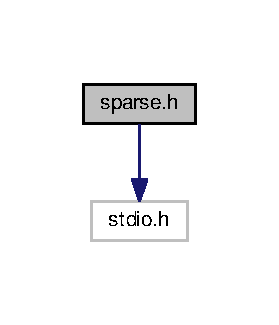
\includegraphics[width=134pt]{sparse_8h__incl}
\end{center}
\end{figure}
Questo grafo mostra quali altri file includono direttamente o indirettamente questo file\+:\nopagebreak
\begin{figure}[H]
\begin{center}
\leavevmode
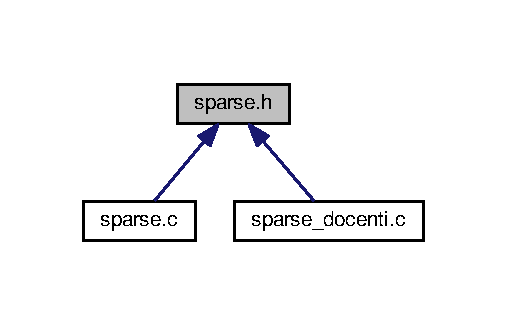
\includegraphics[width=244pt]{sparse_8h__dep__incl}
\end{center}
\end{figure}
\subsection*{Composti}
\begin{DoxyCompactItemize}
\item 
struct \hyperlink{structelem}{elem}
\item 
struct \hyperlink{structsmatrix__t}{smatrix\+\_\+t}
\end{DoxyCompactItemize}
\subsection*{Ridefinizioni di tipo (typedef)}
\begin{DoxyCompactItemize}
\item 
typedef enum \hyperlink{sparse_8h_af6a258d8f3ee5206d682d799316314b1}{bool} \hyperlink{sparse_8h_a4ed992ceefff896353c1727143529d16}{bool\+\_\+t}
\item 
typedef struct \hyperlink{structelem}{elem} \hyperlink{sparse_8h_a14aec81bdea9c2d34b666b7157117387}{elem\+\_\+t}
\end{DoxyCompactItemize}
\subsection*{Tipi enumerati (enum)}
\begin{DoxyCompactItemize}
\item 
enum \hyperlink{sparse_8h_af6a258d8f3ee5206d682d799316314b1}{bool} \{ {\bfseries F\+A\+L\+SE} =0, 
{\bfseries T\+R\+UE} =1
 \}
\end{DoxyCompactItemize}
\subsection*{Funzioni}
\begin{DoxyCompactItemize}
\item 
void \hyperlink{sparse_8h_abe7c306fd1022398d6ee66088635d548}{print\+\_\+smat} (F\+I\+LE $\ast$f, \hyperlink{structsmatrix__t}{smatrix\+\_\+t} $\ast$l)
\item 
\hyperlink{structsmatrix__t}{smatrix\+\_\+t} $\ast$ \hyperlink{sparse_8h_a13f7785dace4a2981b9b6f810ca34115}{new\+\_\+smat} (unsigned n, unsigned m)
\item 
\hyperlink{sparse_8h_a4ed992ceefff896353c1727143529d16}{bool\+\_\+t} \hyperlink{sparse_8h_a4232552afd0fdc736d90fded1f272759}{is\+\_\+equal\+\_\+smat} (\hyperlink{structsmatrix__t}{smatrix\+\_\+t} $\ast$a, \hyperlink{structsmatrix__t}{smatrix\+\_\+t} $\ast$b)
\item 
int \hyperlink{sparse_8h_a098b33ab9b543c109d655b9afc081bb7}{put\+\_\+elem\+\_\+row} (\hyperlink{sparse_8h_a14aec81bdea9c2d34b666b7157117387}{elem\+\_\+t} $\ast$$\ast$r, int j, double d)
\item 
int \hyperlink{sparse_8h_a19ab77e854480bb2c9e5032bc3f0ab9f}{put\+\_\+elem} (\hyperlink{structsmatrix__t}{smatrix\+\_\+t} $\ast$m, unsigned i, unsigned j, double d)
\item 
int \hyperlink{sparse_8h_a23f27b0ac759a8c6cf94ca624a7367d3}{get\+\_\+elem\+\_\+row} (\hyperlink{sparse_8h_a14aec81bdea9c2d34b666b7157117387}{elem\+\_\+t} $\ast$r, int j, double $\ast$pd)
\item 
int \hyperlink{sparse_8h_a03efbfc08da3aa936597103784ddbe45}{get\+\_\+elem} (\hyperlink{structsmatrix__t}{smatrix\+\_\+t} $\ast$m, unsigned i, unsigned j, double $\ast$pd)
\item 
void \hyperlink{sparse_8h_a58e3ead06f0ecc684dfc90538947343a}{free\+\_\+row} (\hyperlink{sparse_8h_a14aec81bdea9c2d34b666b7157117387}{elem\+\_\+t} $\ast$$\ast$pr)
\item 
void \hyperlink{sparse_8h_ad3596ce2e271a24fada5c85f3b8ce0af}{free\+\_\+smat} (\hyperlink{structsmatrix__t}{smatrix\+\_\+t} $\ast$$\ast$pm)
\item 
\hyperlink{structsmatrix__t}{smatrix\+\_\+t} $\ast$ \hyperlink{sparse_8h_afa8c4ca1cb9e4e55f40dd35faa1d9f85}{sum\+\_\+smat} (\hyperlink{structsmatrix__t}{smatrix\+\_\+t} $\ast$a, \hyperlink{structsmatrix__t}{smatrix\+\_\+t} $\ast$b)
\item 
\hyperlink{structsmatrix__t}{smatrix\+\_\+t} $\ast$ \hyperlink{sparse_8h_a633a6b934732ad44f5cf73e9c55c54e9}{prod\+\_\+smat} (\hyperlink{structsmatrix__t}{smatrix\+\_\+t} $\ast$a, \hyperlink{structsmatrix__t}{smatrix\+\_\+t} $\ast$b)
\item 
\hyperlink{structsmatrix__t}{smatrix\+\_\+t} $\ast$ \hyperlink{sparse_8h_a7b9192596db334fe30a652e05ab45987}{transp\+\_\+smat} (\hyperlink{structsmatrix__t}{smatrix\+\_\+t} $\ast$a)
\item 
\hyperlink{structsmatrix__t}{smatrix\+\_\+t} $\ast$ \hyperlink{sparse_8h_ac5049cd89f46bff8cd028382edf931e6}{load\+\_\+smat} (F\+I\+LE $\ast$fd)
\item 
int \hyperlink{sparse_8h_a9ee2597119d106f30a1ba43ba3d6c642}{save\+\_\+smat} (F\+I\+LE $\ast$fd, \hyperlink{structsmatrix__t}{smatrix\+\_\+t} $\ast$mat)
\item 
\hyperlink{structsmatrix__t}{smatrix\+\_\+t} $\ast$ \hyperlink{sparse_8h_a1bb39d59a532967d5f507a19700aafb1}{loadbin\+\_\+smat} (F\+I\+LE $\ast$fd)
\item 
int \hyperlink{sparse_8h_a8529b8bb59f8d259731ef88e5deb6d57}{savebin\+\_\+smat} (F\+I\+LE $\ast$fd, \hyperlink{structsmatrix__t}{smatrix\+\_\+t} $\ast$mat)
\end{DoxyCompactItemize}


\subsection{Descrizione dettagliata}
header file contenente i prototipi da implementare 

\begin{DoxyAuthor}{Autore}
Francesco Lorito 464604 
\end{DoxyAuthor}


\subsection{Documentazione delle ridefinizioni di tipo (typedef)}
\index{sparse.\+h@{sparse.\+h}!bool\+\_\+t@{bool\+\_\+t}}
\index{bool\+\_\+t@{bool\+\_\+t}!sparse.\+h@{sparse.\+h}}
\subsubsection[{\texorpdfstring{bool\+\_\+t}{bool_t}}]{\setlength{\rightskip}{0pt plus 5cm}typedef enum {\bf bool}  {\bf bool\+\_\+t}}\hypertarget{sparse_8h_a4ed992ceefff896353c1727143529d16}{}\label{sparse_8h_a4ed992ceefff896353c1727143529d16}
valori booleani \index{sparse.\+h@{sparse.\+h}!elem\+\_\+t@{elem\+\_\+t}}
\index{elem\+\_\+t@{elem\+\_\+t}!sparse.\+h@{sparse.\+h}}
\subsubsection[{\texorpdfstring{elem\+\_\+t}{elem_t}}]{\setlength{\rightskip}{0pt plus 5cm}typedef struct {\bf elem}  {\bf elem\+\_\+t}}\hypertarget{sparse_8h_a14aec81bdea9c2d34b666b7157117387}{}\label{sparse_8h_a14aec81bdea9c2d34b666b7157117387}
Le matrici sparse di valori double sono rappresentate da un array di liste ciascuna delle quali rappresenta una riga. In ogni lista sono contenuti solo gli elementi non uguali a zero con il numero di colonna corrispondente.

Ad esempio la matrice

3.\+1 0 0 0 0 0 0 0 0 7.\+2 0 9.\+0

è rappresentata come

0 $\vert$ ------$>$(\mbox{[}0,3.\+1\mbox{]} , N\+U\+LL) 1 $\vert$ N\+U\+LL 2 $\vert$ ------$>$(\mbox{[}1,7.\+2\mbox{]} , --)--$>$( \mbox{[}3,9.\+0\mbox{]} ,N\+U\+LL)elemento della matrice sparsa 

\subsection{Documentazione dei tipi enumerati}
\index{sparse.\+h@{sparse.\+h}!bool@{bool}}
\index{bool@{bool}!sparse.\+h@{sparse.\+h}}
\subsubsection[{\texorpdfstring{bool}{bool}}]{\setlength{\rightskip}{0pt plus 5cm}enum {\bf bool}}\hypertarget{sparse_8h_af6a258d8f3ee5206d682d799316314b1}{}\label{sparse_8h_af6a258d8f3ee5206d682d799316314b1}
valori booleani 

\subsection{Documentazione delle funzioni}
\index{sparse.\+h@{sparse.\+h}!free\+\_\+row@{free\+\_\+row}}
\index{free\+\_\+row@{free\+\_\+row}!sparse.\+h@{sparse.\+h}}
\subsubsection[{\texorpdfstring{free\+\_\+row(elem\+\_\+t $\ast$$\ast$pr)}{free_row(elem_t **pr)}}]{\setlength{\rightskip}{0pt plus 5cm}void free\+\_\+row (
\begin{DoxyParamCaption}
\item[{{\bf elem\+\_\+t} $\ast$$\ast$}]{pr}
\end{DoxyParamCaption}
)}\hypertarget{sparse_8h_a58e3ead06f0ecc684dfc90538947343a}{}\label{sparse_8h_a58e3ead06f0ecc684dfc90538947343a}
dealloca tutta la riga di una matrice


\begin{DoxyParams}{Parametri}
{\em pr} & puntatore al putatore della riga da deallocare ($\ast$pr viene messo a N\+U\+LL dalla funzione) \\
\hline
\end{DoxyParams}
\index{sparse.\+h@{sparse.\+h}!free\+\_\+smat@{free\+\_\+smat}}
\index{free\+\_\+smat@{free\+\_\+smat}!sparse.\+h@{sparse.\+h}}
\subsubsection[{\texorpdfstring{free\+\_\+smat(smatrix\+\_\+t $\ast$$\ast$pm)}{free_smat(smatrix_t **pm)}}]{\setlength{\rightskip}{0pt plus 5cm}void free\+\_\+smat (
\begin{DoxyParamCaption}
\item[{{\bf smatrix\+\_\+t} $\ast$$\ast$}]{pm}
\end{DoxyParamCaption}
)}\hypertarget{sparse_8h_ad3596ce2e271a24fada5c85f3b8ce0af}{}\label{sparse_8h_ad3596ce2e271a24fada5c85f3b8ce0af}
dealloca tutta la matrice


\begin{DoxyParams}{Parametri}
{\em pm} & puntatore al putatore della matrice da deallocare ($\ast$pm viene messo a N\+U\+LL dalla funzione) \\
\hline
\end{DoxyParams}
\index{sparse.\+h@{sparse.\+h}!get\+\_\+elem@{get\+\_\+elem}}
\index{get\+\_\+elem@{get\+\_\+elem}!sparse.\+h@{sparse.\+h}}
\subsubsection[{\texorpdfstring{get\+\_\+elem(smatrix\+\_\+t $\ast$m, unsigned i, unsigned j, double $\ast$pd)}{get_elem(smatrix_t *m, unsigned i, unsigned j, double *pd)}}]{\setlength{\rightskip}{0pt plus 5cm}int get\+\_\+elem (
\begin{DoxyParamCaption}
\item[{{\bf smatrix\+\_\+t} $\ast$}]{m, }
\item[{unsigned}]{i, }
\item[{unsigned}]{j, }
\item[{double $\ast$}]{pd}
\end{DoxyParamCaption}
)}\hypertarget{sparse_8h_a03efbfc08da3aa936597103784ddbe45}{}\label{sparse_8h_a03efbfc08da3aa936597103784ddbe45}
legge il valore nell\textquotesingle{}elemento i,j


\begin{DoxyParams}{Parametri}
{\em m} & puntatore alla matrice \\
\hline
{\em (i,j)} & posizione dell\textquotesingle{}elemento \\
\hline
{\em pd} & puntatore della variabile in cui scrivere il valore dell\textquotesingle{}elemento\\
\hline
\end{DoxyParams}

\begin{DoxyRetVals}{Valori di ritorno}
{\em -\/1} & se si e\textquotesingle{} verificato un errore \\
\hline
{\em 0} & altrimenti \\
\hline
\end{DoxyRetVals}
\index{sparse.\+h@{sparse.\+h}!get\+\_\+elem\+\_\+row@{get\+\_\+elem\+\_\+row}}
\index{get\+\_\+elem\+\_\+row@{get\+\_\+elem\+\_\+row}!sparse.\+h@{sparse.\+h}}
\subsubsection[{\texorpdfstring{get\+\_\+elem\+\_\+row(elem\+\_\+t $\ast$r, int j, double $\ast$pd)}{get_elem_row(elem_t *r, int j, double *pd)}}]{\setlength{\rightskip}{0pt plus 5cm}int get\+\_\+elem\+\_\+row (
\begin{DoxyParamCaption}
\item[{{\bf elem\+\_\+t} $\ast$}]{r, }
\item[{int}]{j, }
\item[{double $\ast$}]{pd}
\end{DoxyParamCaption}
)}\hypertarget{sparse_8h_a23f27b0ac759a8c6cf94ca624a7367d3}{}\label{sparse_8h_a23f27b0ac759a8c6cf94ca624a7367d3}
legge il valore dell\textquotesingle{}elemento nella colonna j


\begin{DoxyParams}{Parametri}
{\em r} & puntatore alla riga da leggere \\
\hline
{\em j} & colonna dell\textquotesingle{}elemento \\
\hline
{\em pd} & puntatore della variabile in cui scrivere il valore dell\textquotesingle{}elemento\\
\hline
\end{DoxyParams}

\begin{DoxyRetVals}{Valori di ritorno}
{\em -\/1} & se si e\textquotesingle{} verificato un errore \\
\hline
{\em 0} & altrimenti \\
\hline
\end{DoxyRetVals}
\index{sparse.\+h@{sparse.\+h}!is\+\_\+equal\+\_\+smat@{is\+\_\+equal\+\_\+smat}}
\index{is\+\_\+equal\+\_\+smat@{is\+\_\+equal\+\_\+smat}!sparse.\+h@{sparse.\+h}}
\subsubsection[{\texorpdfstring{is\+\_\+equal\+\_\+smat(smatrix\+\_\+t $\ast$a, smatrix\+\_\+t $\ast$b)}{is_equal_smat(smatrix_t *a, smatrix_t *b)}}]{\setlength{\rightskip}{0pt plus 5cm}{\bf bool\+\_\+t} is\+\_\+equal\+\_\+smat (
\begin{DoxyParamCaption}
\item[{{\bf smatrix\+\_\+t} $\ast$}]{a, }
\item[{{\bf smatrix\+\_\+t} $\ast$}]{b}
\end{DoxyParamCaption}
)}\hypertarget{sparse_8h_a4232552afd0fdc736d90fded1f272759}{}\label{sparse_8h_a4232552afd0fdc736d90fded1f272759}
Controlla se due matrici sono uguali, elemento per elemento


\begin{DoxyParams}{Parametri}
{\em a} & puntatore alla prima matrice da confrontare \\
\hline
{\em b} & puntatore alla seconda matrice da confrontare\\
\hline
\end{DoxyParams}

\begin{DoxyRetVals}{Valori di ritorno}
{\em T\+R\+UE} & se sono uguali \\
\hline
{\em F\+A\+L\+SE} & altrimenti \\
\hline
\end{DoxyRetVals}
\index{sparse.\+h@{sparse.\+h}!load\+\_\+smat@{load\+\_\+smat}}
\index{load\+\_\+smat@{load\+\_\+smat}!sparse.\+h@{sparse.\+h}}
\subsubsection[{\texorpdfstring{load\+\_\+smat(\+F\+I\+L\+E $\ast$fd)}{load_smat(FILE *fd)}}]{\setlength{\rightskip}{0pt plus 5cm}{\bf smatrix\+\_\+t}$\ast$ load\+\_\+smat (
\begin{DoxyParamCaption}
\item[{F\+I\+LE $\ast$}]{fd}
\end{DoxyParamCaption}
)}\hypertarget{sparse_8h_ac5049cd89f46bff8cd028382edf931e6}{}\label{sparse_8h_ac5049cd89f46bff8cd028382edf931e6}
carica da file una matrice nel formato nrighe1 ncolonne1 riga1 colonna1 valore1 ... rigaN colonnaN valoreN

Ad esempio la matrice

3.\+1 0 0 0 0 0 0 0 0 7.\+2 0 9.\+0

è rappresentata come 3 3 0 0 3.\+1 2 1 7.\+2 2 2 9.\+0


\begin{DoxyParams}{Parametri}
{\em fd} & file da cui caricare la matrice (gia\textquotesingle{} aperto)\\
\hline
\end{DoxyParams}

\begin{DoxyRetVals}{Valori di ritorno}
{\em p} & puntatore alla nuove matrice caricata (allocata dentro la funzione) \\
\hline
{\em N\+U\+LL} & se si è verificato un errore (setta errno) \\
\hline
\end{DoxyRetVals}
\index{sparse.\+h@{sparse.\+h}!loadbin\+\_\+smat@{loadbin\+\_\+smat}}
\index{loadbin\+\_\+smat@{loadbin\+\_\+smat}!sparse.\+h@{sparse.\+h}}
\subsubsection[{\texorpdfstring{loadbin\+\_\+smat(\+F\+I\+L\+E $\ast$fd)}{loadbin_smat(FILE *fd)}}]{\setlength{\rightskip}{0pt plus 5cm}{\bf smatrix\+\_\+t}$\ast$ loadbin\+\_\+smat (
\begin{DoxyParamCaption}
\item[{F\+I\+LE $\ast$}]{fd}
\end{DoxyParamCaption}
)}\hypertarget{sparse_8h_a1bb39d59a532967d5f507a19700aafb1}{}\label{sparse_8h_a1bb39d59a532967d5f507a19700aafb1}
carica da file una matrice in formato binario (scelto dallo studente e documentato nei commenti) \begin{DoxyVerb}Il file binario si presenta come un'unica stringa di bit
    110010101110..............010101

i primi sizeof(int) bit  indicano il numrow
i secondi sizeof(int) bit  indicano il numcol
i successivi bit indicano il contenuto della matrice esono disposti come segue:
    un blocco di sizeof(int) per l'indice di riga
    un blocco di sizeof(int) per l'indice di colonna
    e un blocco di sizeof(double) per il valore dell'elemento
e così via per ogni elemento della matrice
\end{DoxyVerb}



\begin{DoxyParams}{Parametri}
{\em fd} & file da cui caricare la matrice (gia\textquotesingle{} aperto)\\
\hline
\end{DoxyParams}

\begin{DoxyRetVals}{Valori di ritorno}
{\em p} & puntatore alla nuove matrice caricata (allocata dentro la funzione) \\
\hline
{\em N\+U\+LL} & se si è verificato un errore (setta errno) \\
\hline
\end{DoxyRetVals}
\index{sparse.\+h@{sparse.\+h}!new\+\_\+smat@{new\+\_\+smat}}
\index{new\+\_\+smat@{new\+\_\+smat}!sparse.\+h@{sparse.\+h}}
\subsubsection[{\texorpdfstring{new\+\_\+smat(unsigned n, unsigned m)}{new_smat(unsigned n, unsigned m)}}]{\setlength{\rightskip}{0pt plus 5cm}{\bf smatrix\+\_\+t}$\ast$ new\+\_\+smat (
\begin{DoxyParamCaption}
\item[{unsigned}]{n, }
\item[{unsigned}]{m}
\end{DoxyParamCaption}
)}\hypertarget{sparse_8h_a13f7785dace4a2981b9b6f810ca34115}{}\label{sparse_8h_a13f7785dace4a2981b9b6f810ca34115}
crea una nuova matrice vuota 
\begin{DoxyParams}{Parametri}
{\em n} & numero di righe \\
\hline
{\em m} & numero di colonne\\
\hline
\end{DoxyParams}

\begin{DoxyRetVals}{Valori di ritorno}
{\em N\+U\+LL} & se si e\textquotesingle{} verificato un errore \\
\hline
{\em p} & ppuntatore alla matrice appena allocata \\
\hline
\end{DoxyRetVals}
\index{sparse.\+h@{sparse.\+h}!print\+\_\+smat@{print\+\_\+smat}}
\index{print\+\_\+smat@{print\+\_\+smat}!sparse.\+h@{sparse.\+h}}
\subsubsection[{\texorpdfstring{print\+\_\+smat(\+F\+I\+L\+E $\ast$f, smatrix\+\_\+t $\ast$l)}{print_smat(FILE *f, smatrix_t *l)}}]{\setlength{\rightskip}{0pt plus 5cm}void print\+\_\+smat (
\begin{DoxyParamCaption}
\item[{F\+I\+LE $\ast$}]{f, }
\item[{{\bf smatrix\+\_\+t} $\ast$}]{l}
\end{DoxyParamCaption}
)}\hypertarget{sparse_8h_abe7c306fd1022398d6ee66088635d548}{}\label{sparse_8h_abe7c306fd1022398d6ee66088635d548}
stampa la matrice in forma canonica (F\+O\+R\+N\+I\+TA D\+AI D\+O\+C\+E\+N\+TI)


\begin{DoxyParams}{Parametri}
{\em l} & putatore alla matrice da stampare \\
\hline
{\em f} & puntatore al file su cui scrivere \\
\hline
\end{DoxyParams}
\index{sparse.\+h@{sparse.\+h}!prod\+\_\+smat@{prod\+\_\+smat}}
\index{prod\+\_\+smat@{prod\+\_\+smat}!sparse.\+h@{sparse.\+h}}
\subsubsection[{\texorpdfstring{prod\+\_\+smat(smatrix\+\_\+t $\ast$a, smatrix\+\_\+t $\ast$b)}{prod_smat(smatrix_t *a, smatrix_t *b)}}]{\setlength{\rightskip}{0pt plus 5cm}{\bf smatrix\+\_\+t}$\ast$ prod\+\_\+smat (
\begin{DoxyParamCaption}
\item[{{\bf smatrix\+\_\+t} $\ast$}]{a, }
\item[{{\bf smatrix\+\_\+t} $\ast$}]{b}
\end{DoxyParamCaption}
)}\hypertarget{sparse_8h_a633a6b934732ad44f5cf73e9c55c54e9}{}\label{sparse_8h_a633a6b934732ad44f5cf73e9c55c54e9}
moltiplica due matrici (se il prodotto è zero ricordarsi di non inserire l\textquotesingle{}elemento corrispondente) 
\begin{DoxyParams}{Parametri}
{\em a,b} & matrici da moltiplicare\\
\hline
\end{DoxyParams}

\begin{DoxyRetVals}{Valori di ritorno}
{\em c} & la matrice risultato (viene allocata dentro la funzione) \\
\hline
{\em N\+U\+LL} & se si è verificato un errore \\
\hline
\end{DoxyRetVals}
\index{sparse.\+h@{sparse.\+h}!put\+\_\+elem@{put\+\_\+elem}}
\index{put\+\_\+elem@{put\+\_\+elem}!sparse.\+h@{sparse.\+h}}
\subsubsection[{\texorpdfstring{put\+\_\+elem(smatrix\+\_\+t $\ast$m, unsigned i, unsigned j, double d)}{put_elem(smatrix_t *m, unsigned i, unsigned j, double d)}}]{\setlength{\rightskip}{0pt plus 5cm}int put\+\_\+elem (
\begin{DoxyParamCaption}
\item[{{\bf smatrix\+\_\+t} $\ast$}]{m, }
\item[{unsigned}]{i, }
\item[{unsigned}]{j, }
\item[{double}]{d}
\end{DoxyParamCaption}
)}\hypertarget{sparse_8h_a19ab77e854480bb2c9e5032bc3f0ab9f}{}\label{sparse_8h_a19ab77e854480bb2c9e5032bc3f0ab9f}
scrive un valore nell\textquotesingle{}elemento i,j, per mantenere la rappresentazione consistente se il valore scritto è 0 l\textquotesingle{}elemento corrispondente deve essere eliminato dalla lista che rappresenta la riga


\begin{DoxyParams}{Parametri}
{\em m} & puntatore alla matrice \\
\hline
{\em (i,j)} & posizione dell\textquotesingle{}elemento \\
\hline
{\em d} & valore dell\textquotesingle{}elemento da scrivere\\
\hline
\end{DoxyParams}

\begin{DoxyRetVals}{Valori di ritorno}
{\em -\/1} & se si e\textquotesingle{} verificato un errore \\
\hline
{\em 0} & altrimenti \\
\hline
\end{DoxyRetVals}
\index{sparse.\+h@{sparse.\+h}!put\+\_\+elem\+\_\+row@{put\+\_\+elem\+\_\+row}}
\index{put\+\_\+elem\+\_\+row@{put\+\_\+elem\+\_\+row}!sparse.\+h@{sparse.\+h}}
\subsubsection[{\texorpdfstring{put\+\_\+elem\+\_\+row(elem\+\_\+t $\ast$$\ast$r, int j, double d)}{put_elem_row(elem_t **r, int j, double d)}}]{\setlength{\rightskip}{0pt plus 5cm}int put\+\_\+elem\+\_\+row (
\begin{DoxyParamCaption}
\item[{{\bf elem\+\_\+t} $\ast$$\ast$}]{r, }
\item[{int}]{j, }
\item[{double}]{d}
\end{DoxyParamCaption}
)}\hypertarget{sparse_8h_a098b33ab9b543c109d655b9afc081bb7}{}\label{sparse_8h_a098b33ab9b543c109d655b9afc081bb7}
inserisce un elemento in r passata con indice colonna j, per mantenere la rappresentazione consistente se il valore scritto è 0 l\textquotesingle{}elemento corrispondente deve essere eliminato dalla lista che rappresenta la riga


\begin{DoxyParams}{Parametri}
{\em r} & puntatore alla riga \\
\hline
{\em j} & colonna dell\textquotesingle{}elemento \\
\hline
{\em d} & valore dell\textquotesingle{}elemento da scrivere\\
\hline
\end{DoxyParams}

\begin{DoxyRetVals}{Valori di ritorno}
{\em -\/1} & se si e\textquotesingle{} verificato un errore \\
\hline
{\em 0} & altrimenti \\
\hline
\end{DoxyRetVals}
\index{sparse.\+h@{sparse.\+h}!save\+\_\+smat@{save\+\_\+smat}}
\index{save\+\_\+smat@{save\+\_\+smat}!sparse.\+h@{sparse.\+h}}
\subsubsection[{\texorpdfstring{save\+\_\+smat(\+F\+I\+L\+E $\ast$fd, smatrix\+\_\+t $\ast$mat)}{save_smat(FILE *fd, smatrix_t *mat)}}]{\setlength{\rightskip}{0pt plus 5cm}int save\+\_\+smat (
\begin{DoxyParamCaption}
\item[{F\+I\+LE $\ast$}]{fd, }
\item[{{\bf smatrix\+\_\+t} $\ast$}]{mat}
\end{DoxyParamCaption}
)}\hypertarget{sparse_8h_a9ee2597119d106f30a1ba43ba3d6c642}{}\label{sparse_8h_a9ee2597119d106f30a1ba43ba3d6c642}
salva una matrice su file nel formato specificato per la funzione load\+\_\+smat


\begin{DoxyParams}{Parametri}
{\em fd} & file su cui scrivere la matrice (gia\textquotesingle{} aperto) \\
\hline
{\em mat} & la matrice da scrivere su file\\
\hline
\end{DoxyParams}

\begin{DoxyRetVals}{Valori di ritorno}
{\em 0} & se tutto e\textquotesingle{} andato bene \\
\hline
{\em -\/1} & se si è verificato un errore (setta errno) \\
\hline
\end{DoxyRetVals}
\index{sparse.\+h@{sparse.\+h}!savebin\+\_\+smat@{savebin\+\_\+smat}}
\index{savebin\+\_\+smat@{savebin\+\_\+smat}!sparse.\+h@{sparse.\+h}}
\subsubsection[{\texorpdfstring{savebin\+\_\+smat(\+F\+I\+L\+E $\ast$fd, smatrix\+\_\+t $\ast$mat)}{savebin_smat(FILE *fd, smatrix_t *mat)}}]{\setlength{\rightskip}{0pt plus 5cm}int savebin\+\_\+smat (
\begin{DoxyParamCaption}
\item[{F\+I\+LE $\ast$}]{fd, }
\item[{{\bf smatrix\+\_\+t} $\ast$}]{mat}
\end{DoxyParamCaption}
)}\hypertarget{sparse_8h_a8529b8bb59f8d259731ef88e5deb6d57}{}\label{sparse_8h_a8529b8bb59f8d259731ef88e5deb6d57}
salva una matrice su file in formato binario (scelto dallo studente e documentato nei commenti) \mbox{[}stesso formato documentato in loadbin\+\_\+smat\mbox{]}


\begin{DoxyParams}{Parametri}
{\em fd} & file su cui scrivere la matrice (gia\textquotesingle{} aperto) \\
\hline
{\em mat} & la matrice da scrivere su file\\
\hline
\end{DoxyParams}

\begin{DoxyRetVals}{Valori di ritorno}
{\em 0} & se tutto e\textquotesingle{} andato bene \\
\hline
{\em -\/1} & se si è verificato un errore (setta errno) \\
\hline
\end{DoxyRetVals}
\index{sparse.\+h@{sparse.\+h}!sum\+\_\+smat@{sum\+\_\+smat}}
\index{sum\+\_\+smat@{sum\+\_\+smat}!sparse.\+h@{sparse.\+h}}
\subsubsection[{\texorpdfstring{sum\+\_\+smat(smatrix\+\_\+t $\ast$a, smatrix\+\_\+t $\ast$b)}{sum_smat(smatrix_t *a, smatrix_t *b)}}]{\setlength{\rightskip}{0pt plus 5cm}{\bf smatrix\+\_\+t}$\ast$ sum\+\_\+smat (
\begin{DoxyParamCaption}
\item[{{\bf smatrix\+\_\+t} $\ast$}]{a, }
\item[{{\bf smatrix\+\_\+t} $\ast$}]{b}
\end{DoxyParamCaption}
)}\hypertarget{sparse_8h_afa8c4ca1cb9e4e55f40dd35faa1d9f85}{}\label{sparse_8h_afa8c4ca1cb9e4e55f40dd35faa1d9f85}
somma due matrici (se la somma è zero ricordarsi di non inserire l\textquotesingle{}elemento corrispondente) 
\begin{DoxyParams}{Parametri}
{\em a,b} & matrici da sommare\\
\hline
\end{DoxyParams}

\begin{DoxyRetVals}{Valori di ritorno}
{\em c} & la matrice risultato (viene allocata dentro la funzione) \\
\hline
{\em N\+U\+LL} & se si è verificato un errore \\
\hline
\end{DoxyRetVals}
\index{sparse.\+h@{sparse.\+h}!transp\+\_\+smat@{transp\+\_\+smat}}
\index{transp\+\_\+smat@{transp\+\_\+smat}!sparse.\+h@{sparse.\+h}}
\subsubsection[{\texorpdfstring{transp\+\_\+smat(smatrix\+\_\+t $\ast$a)}{transp_smat(smatrix_t *a)}}]{\setlength{\rightskip}{0pt plus 5cm}{\bf smatrix\+\_\+t}$\ast$ transp\+\_\+smat (
\begin{DoxyParamCaption}
\item[{{\bf smatrix\+\_\+t} $\ast$}]{a}
\end{DoxyParamCaption}
)}\hypertarget{sparse_8h_a7b9192596db334fe30a652e05ab45987}{}\label{sparse_8h_a7b9192596db334fe30a652e05ab45987}
calcola la trasposta di una matrice (se un elemento è zero ricordarsi di non inserire) 
\begin{DoxyParams}{Parametri}
{\em a} & matrice\\
\hline
\end{DoxyParams}

\begin{DoxyRetVals}{Valori di ritorno}
{\em c} & la matrice risultato (viene allocata dentro la funzione) \\
\hline
{\em N\+U\+LL} & se si è verificato un errore \\
\hline
\end{DoxyRetVals}

\hypertarget{sparse__docenti_8c}{}\section{Riferimenti per il file sparse\+\_\+docenti.\+c}
\label{sparse__docenti_8c}\index{sparse\+\_\+docenti.\+c@{sparse\+\_\+docenti.\+c}}


funzioni print smat implementata dai docenti  


{\ttfamily \#include $<$stdio.\+h$>$}\\*
{\ttfamily \#include $<$stdlib.\+h$>$}\\*
{\ttfamily \#include \char`\"{}sparse.\+h\char`\"{}}\\*
Grafo delle dipendenze di inclusione per sparse\+\_\+docenti.\+c\+:
\nopagebreak
\begin{figure}[H]
\begin{center}
\leavevmode
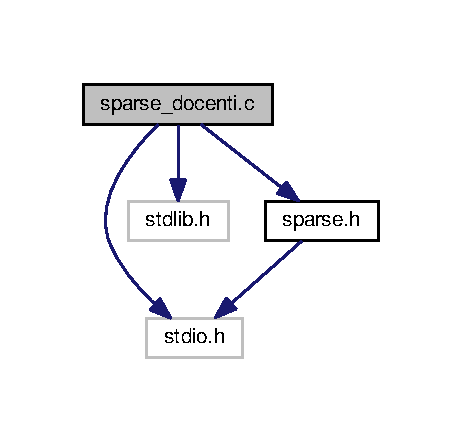
\includegraphics[width=222pt]{sparse__docenti_8c__incl}
\end{center}
\end{figure}
\subsection*{Funzioni}
\begin{DoxyCompactItemize}
\item 
void \hyperlink{sparse__docenti_8c_a908b6cb8261c0131e8c71d842a4381c1}{print\+\_\+smat} (F\+I\+LE $\ast$f, \hyperlink{structsmatrix__t}{smatrix\+\_\+t} $\ast$a)
\end{DoxyCompactItemize}


\subsection{Descrizione dettagliata}
funzioni print smat implementata dai docenti 

\begin{DoxyAuthor}{Autore}
Docenti Sol Lab 2015/2016 
\end{DoxyAuthor}


\subsection{Documentazione delle funzioni}
\index{sparse\+\_\+docenti.\+c@{sparse\+\_\+docenti.\+c}!print\+\_\+smat@{print\+\_\+smat}}
\index{print\+\_\+smat@{print\+\_\+smat}!sparse\+\_\+docenti.\+c@{sparse\+\_\+docenti.\+c}}
\subsubsection[{\texorpdfstring{print\+\_\+smat(\+F\+I\+L\+E $\ast$f, smatrix\+\_\+t $\ast$a)}{print_smat(FILE *f, smatrix_t *a)}}]{\setlength{\rightskip}{0pt plus 5cm}void print\+\_\+smat (
\begin{DoxyParamCaption}
\item[{F\+I\+LE $\ast$}]{f, }
\item[{{\bf smatrix\+\_\+t} $\ast$}]{l}
\end{DoxyParamCaption}
)}\hypertarget{sparse__docenti_8c_a908b6cb8261c0131e8c71d842a4381c1}{}\label{sparse__docenti_8c_a908b6cb8261c0131e8c71d842a4381c1}
stampa la matrice in forma canonica (F\+O\+R\+N\+I\+TA D\+AI D\+O\+C\+E\+N\+TI)


\begin{DoxyParams}{Parametri}
{\em l} & putatore alla matrice da stampare \\
\hline
{\em f} & puntatore al file su cui scrivere \\
\hline
\end{DoxyParams}

%--- End generated contents ---

% Index
\backmatter
\newpage
\phantomsection
\clearemptydoublepage
\addcontentsline{toc}{chapter}{Indice}
\printindex

\end{document}
